\section{Análisis de Color}

Para analizar este atributo, emplearemos el algoritmo de segmentación. No obstante, con el fin de mejorar su rendimiento, se implementará una versión que no requiera la introducción manual del número de clústers. Hasta este punto, todas las imágenes se han segmentado utilizando 15 clústeres; no obstante, más adelante llevaremos a cabo una comparativa entre el valor original y el número óptimo obtenido con este nuevo método.


\subsection{Selección óptima de clústeres con el método del Codo}

El método del codo es una técnica gráfica utilizada para determinar el número óptimo de clústeres (K) en el algoritmo de agrupamiento K-means. Este método se basa en la búsqueda de la suma de los cuadrados intra-cluster (WCSS, por sus siglas en inglés), que representa la suma de las distancias al cuadrado entre los puntos de un clúster y el centroide de ese clúster \autocite{Zheng:2018}.

En el proceso de K-means, se prueban diferentes valores de K para dividir el conjunto de datos en un número específico de clústeres. Para cada valor de K, se calcula el WCSS. El WCSS disminuirá a medida que aumente K, ya que cada punto estará más cerca de su centroide en clústeres más pequeños \autocite{Anju:2019}. Sin embargo, llegará un punto en el que el incremento adicional en K no conllevará una reducción significativa en el WCSS \autocite{Dhanachandra:2015}.

La representación gráfica de esta relación entre el número de clústeres y el WCSS se asemeja a la forma de un ''codo'' en una gráfica, como se puede observar en la figura dieciocho. El punto en el que se observa una desaceleración en la disminución del WCSS y la curva parece formar un codo es considerado como el número óptimo de clústeres para el conjunto de \autocite{Sammouda:2021}. Para la implementación de este algoritmo se define una función que recibe tres parámetros:

\begin{itemize}
    \item originalImage: imagen original que se utilizará para el análisis.
    \item maxClusters: número máximo de clústers que se probarán. En este caso, todas las imágenes tendrán con máximo 15 unidades, para una mejor comparativa con los resultados originales.
    \item maxIter: número máximo de iteraciones para el algoritmo de k-means en cada prueba de clúster.
\end{itemize}

\noindent Dentro de la función se realizan las siguientes operaciones:

\begin{itemize}
    \item Convertimos la imagen original en una matriz de dos dimensiones y se normaliza dividiendo cada valor por 255.
    \item Obtener el número de píxeles con la función numel
    \item Mediante un ciclo for sobre el rango de clústers desde 1 hasta maxClusters. Para cada número de clústers, se inicializan centroides de clústeres de manera aleatoria con ayuda de randperm.
    \item Se ejecuta el algoritmo de k-means en maxIter iteraciones.
    \item La distorsión, que es la suma de los cuadrados de las distancias mínimas al cuadrado se calcula y almacena para evaluar la ''calidad'' del agrupamiento.

     \begin{lstlisting}[style=Matlab-editor, caption=Fragmento del algoritmo findOptimalCluster, basicstyle=\fontsize{8}{12}\selectfont]
for k = 1:maxClusters
    randIndices = randperm(pixelNo, k);
    centers = im2(randIndices);

    for iter = 1:maxIter
        D = pdist2(centers, im2);
       [~, min_indices] = min(D);

        for j = 1:k
            centers(j) = mean(im2(min_indices == j));
        end
    end

    distortions(k) = sum(min(D).^2) / pixelNo;
end
\end{lstlisting}

    \item Se gráfican los resultados obtenidos de la distorsión, se encuentra el codo de los resultados con la primera derivada. Para esto se usa una función adicional 'findKnee'

\begin{lstlisting}[style=Matlab-editor, caption=Algoritmo findKnee, basicstyle=\fontsize{8}{12}\selectfont]
function [x, y] = findKnee(xValues)
    dx = xValues(2:end) - xValues(1:end-1);
    dy = diff(dx);
    [~, idx] = max(dy); 
    x = idx + 1;  
    y = xValues(x);
end
\end{lstlisting}

\end{itemize}


\begin{figure}
		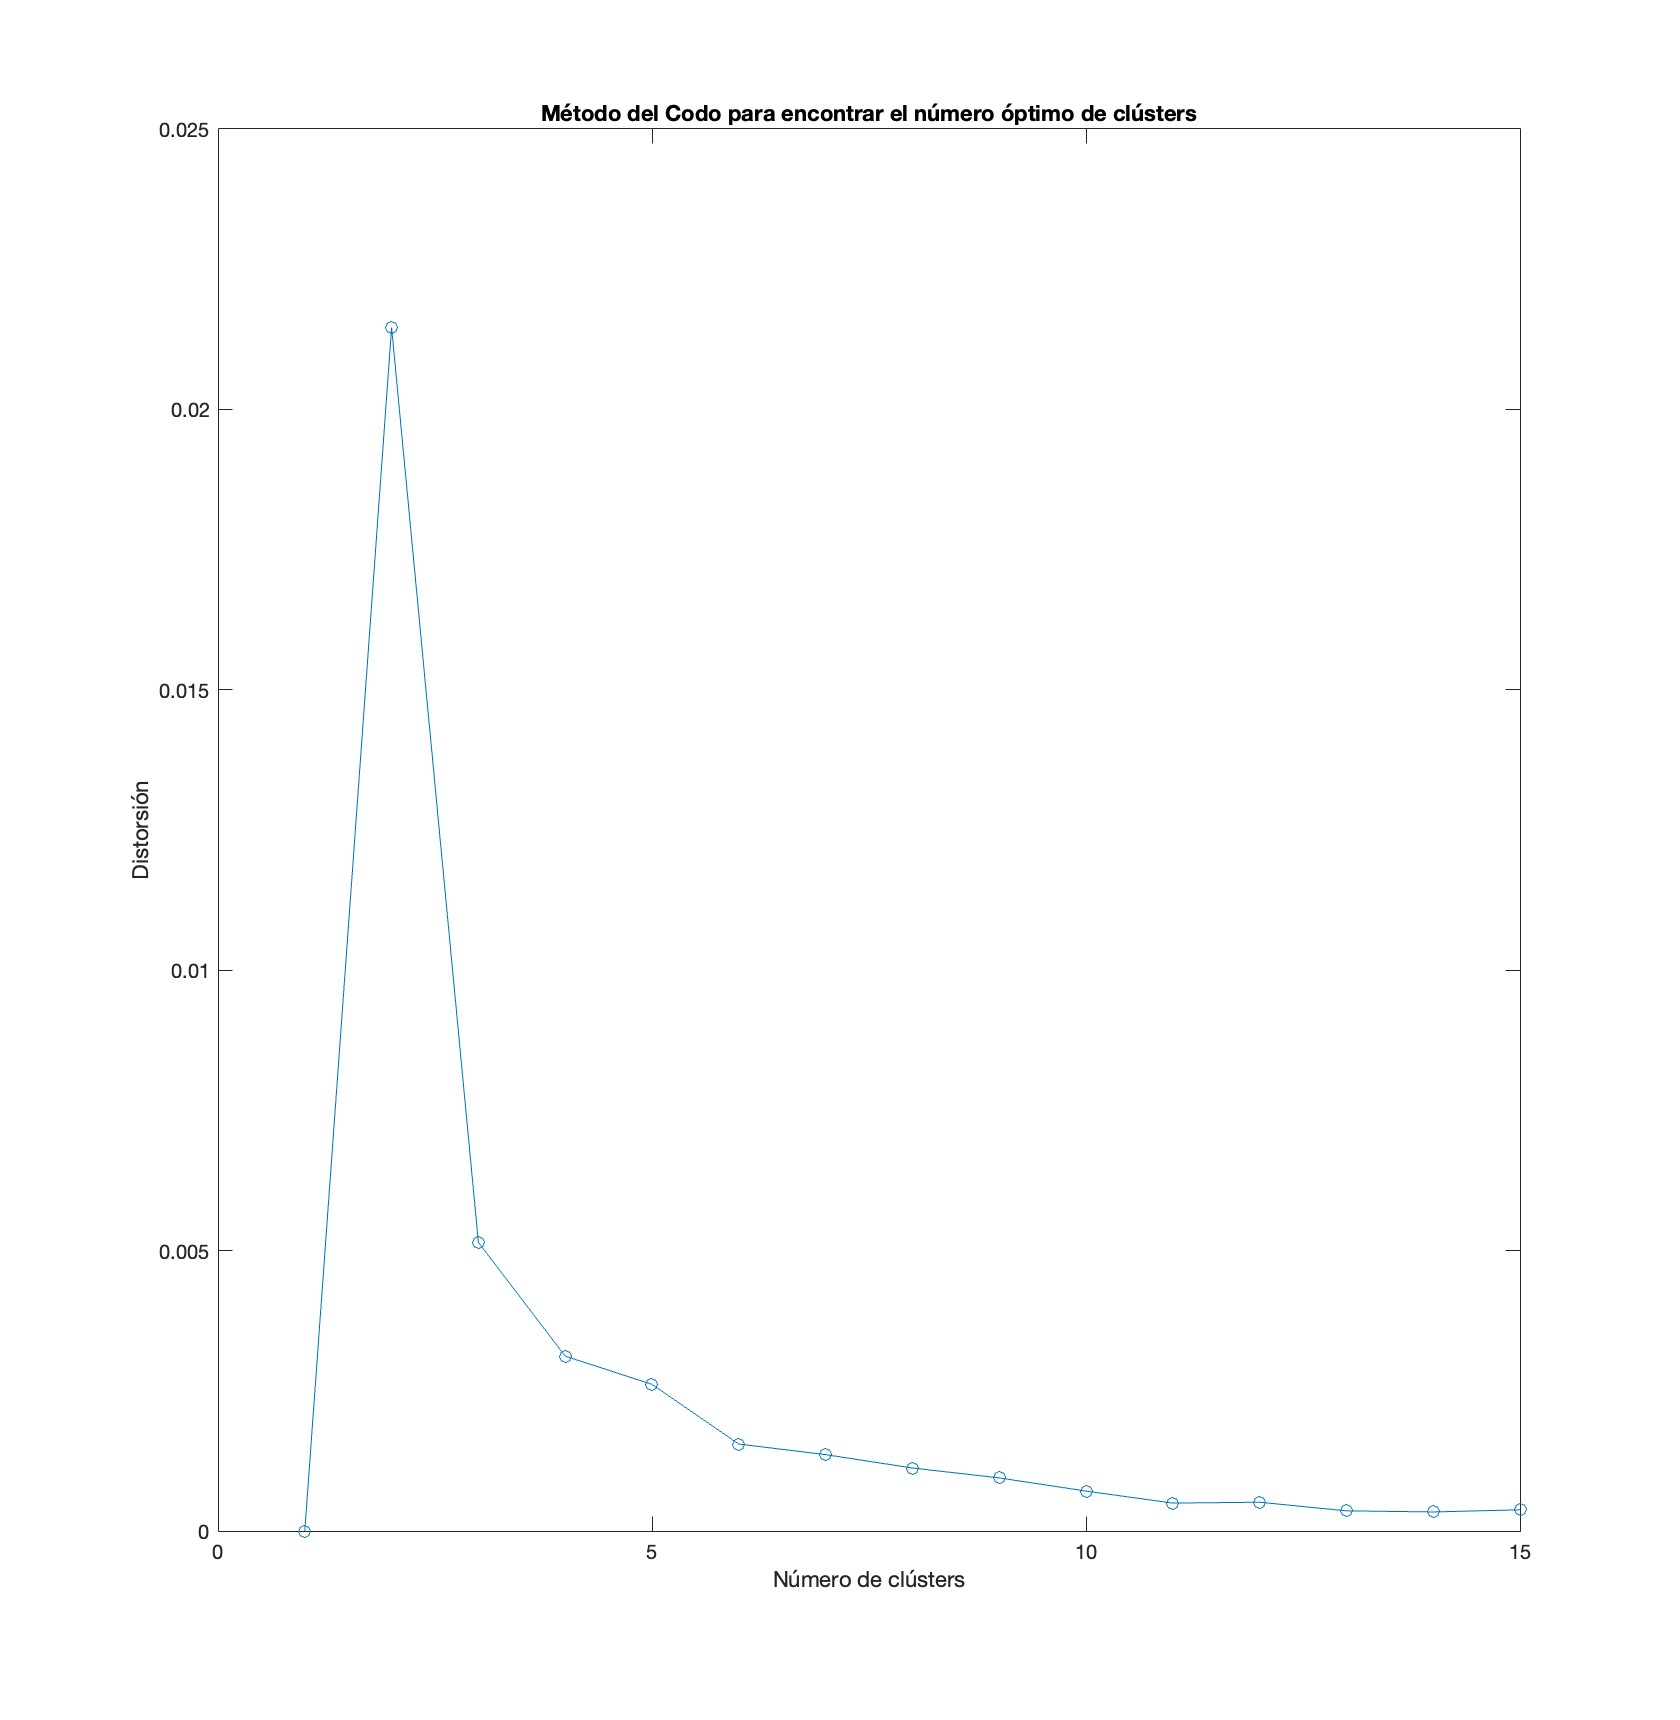
\includegraphics[width=8cm]{images/F18.jpg} 
\caption{Gráfica para evaluar el número óptimo de clústers. Sobre el eje horizontal se encuentra el número de clústers, el eje vertical muestra la desviación sobre el valor K. En este caso el bajo el método del codo el número óptimo es cinco.}
\label{fig18}
\end{figure}

En (Figura~\ref{fig19}) se presenta una comparativa con la selección óptima de clústeres, donde se destaca el rendimiento satisfactorio cuando hay un número elevado de clústeres y cuando se segmenta con el valor óptimo. No obstante, se muestra que al incrementar este valor tareas como la segmentación por color o la compresión de imágenes se ven afectadas. No solo eso, mediante el método del codo se logran conservar los atributos necesarios para resaltar los bordes con una reducción considerable de información. Los resultados de este análisis abarcan desde la (Figura \ref{fig22}) hasta la (Figura \ref{fig26}).


% Figura 19
\begin{figure}[h] 
\begin{tabular}{cc}
    \textbf{15 clústers} & \textbf{Óptimo: 5} \\
    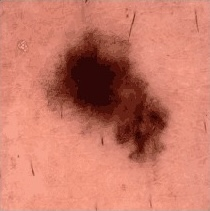
\includegraphics[width=1.7cm]{images/F19-A.jpg} &
    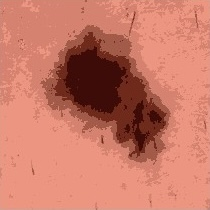
\includegraphics[width=1.7cm]{images/F19-B.jpg} \\
    \textbf{15 clústers} & \textbf{Óptimo: 5} \\
    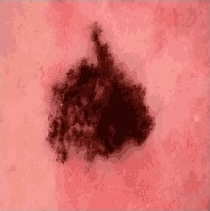
\includegraphics[width=1.7cm]{images/F19-C.jpg} & 
    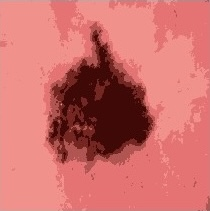
\includegraphics[width=1.7cm]{images/F19-D.jpg} \\
	\textbf{15 clústers} & \textbf{Óptimo: 3} \\
    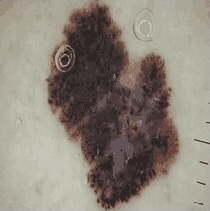
\includegraphics[width=1.7cm]{images/F19-E.jpg} &
    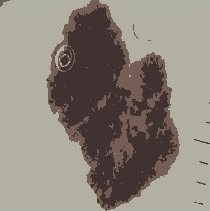
\includegraphics[width=1.7cm]{images/F19-F.jpg} \\
	\textbf{15 clústers} & \textbf{Óptimo: 6} \\
    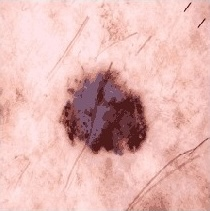
\includegraphics[width=1.7cm]{images/F19-G.jpg} & 
    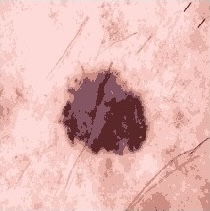
\includegraphics[width=1.7cm]{images/F19-H.jpg} \\
	\textbf{15 clústers} & \textbf{Óptimo: 5} \\
	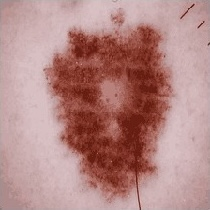
\includegraphics[width=1.7cm]{images/F19-I.jpg} & 
    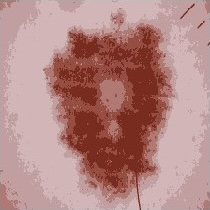
\includegraphics[width=1.7cm]{images/F19-J.jpg} \\
\end{tabular}
\caption{Comparación de uso con selección óptima de clústeres: las imá- genes en la columna izquierda fueron segmentadas con 15 clústers, mientras que las de la derecha utilizaron un valor obtenido mediante el método del codo, indicando en su etiqueta el número de clústers}  
\label{fig19} 
\end{figure}

La figura diseñada para el análisis de color, presenta cada uno de los colores segregados de la imagen original en una única fila utilizando el método para obtener el método óptimo de clústers. Para un análisis más enriquecedor, se decide mostrar los colores segmentados con dos fondos distintos: blanco y negro. Ambos resultados pueden verse en   (Figura~\ref{fig20}) y (Figura~\ref{fig21}). 

% Figura 20
\begin{figure}
    \centering
    \begin{tabular}{ccccc}
        \adjustbox{valign=c}{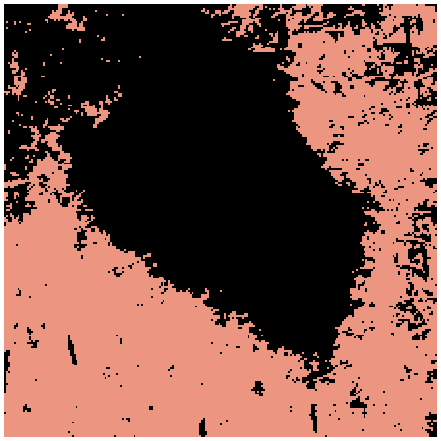
\includegraphics[width=1.3cm]{images/F20-A.png}} &
        \adjustbox{valign=c}{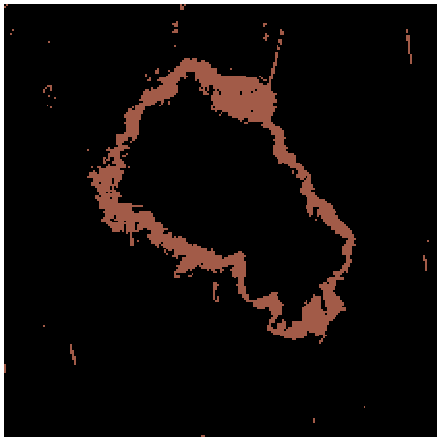
\includegraphics[width=1.3cm]{images/F20-B.png}} & 
        \adjustbox{valign=c}{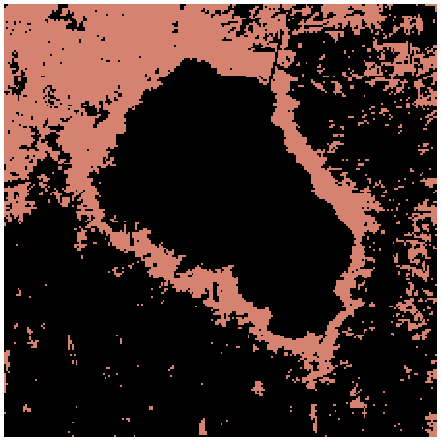
\includegraphics[width=1.3cm]{images/F20-C.png}} & 
		\adjustbox{valign=c}{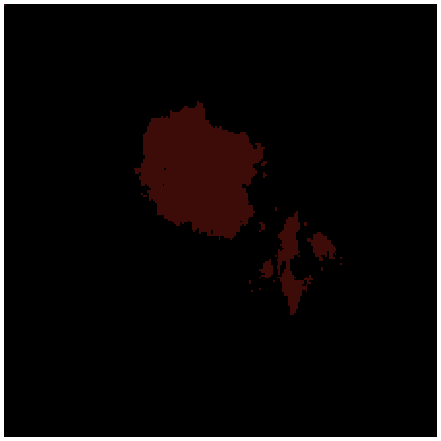
\includegraphics[width=1.3cm]{images/F20-D.png}} & 
        \adjustbox{valign=c}{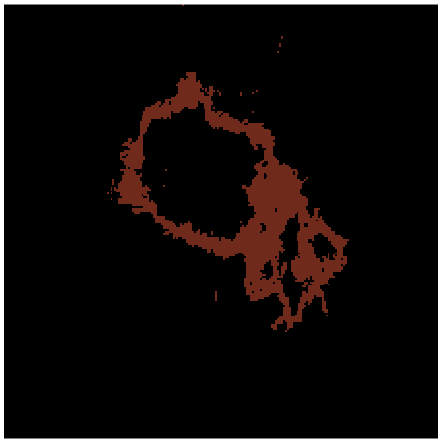
\includegraphics[width=1.3cm]{images/F20-E.png}} \\
        (a) & (b) & (c) & (d) & (e)\\
    \end{tabular}
    \caption{\footnotesize Colores segmentados de la imagen original con el método del codo, el área que no corresponde al color segmentado se aprecia de color negro.}  
    \label{fig20} 
\end{figure}

% Figura 21
\begin{figure}
    \centering
    \begin{tabular}{ccccc}
        \adjustbox{valign=c}{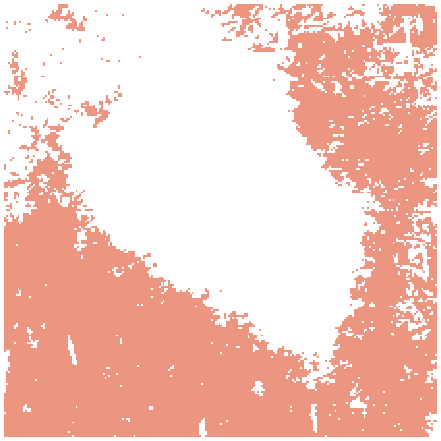
\includegraphics[width=1.3cm]{images/F21-A.png}} &
        \adjustbox{valign=c}{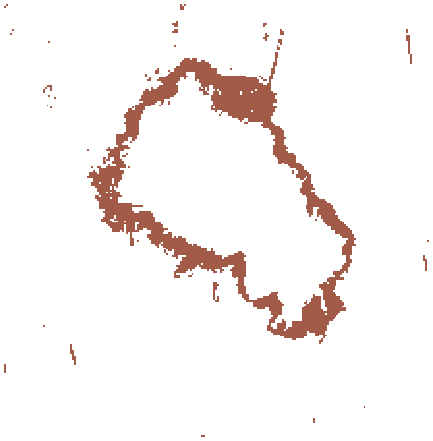
\includegraphics[width=1.3cm]{images/F21-B.png}} & 
        \adjustbox{valign=c}{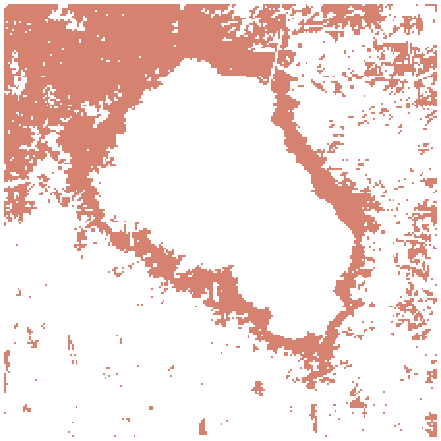
\includegraphics[width=1.3cm]{images/F21-C.png}} & 
		\adjustbox{valign=c}{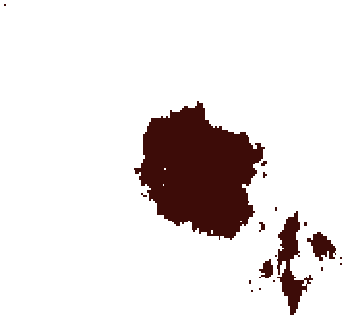
\includegraphics[width=1.3cm]{images/F21-D.png}} & 
        \adjustbox{valign=c}{
\includegraphics[width=1.3cm]{images/F21-E.png}} \\
        (a) & (b) & (c) & (d) & (e) \\
    \end{tabular}
    \caption{\footnotesize Colores segmentados de la imagen original con el método del codo, el área que no corresponde al color segmentado se aprecia de color blanco.}  
    \label{fig21} 
\end{figure}


% FIGURA 22
\begin{figure*}
    \centering
    \begin{tabular}{cccccc}
        \adjustbox{valign=c}{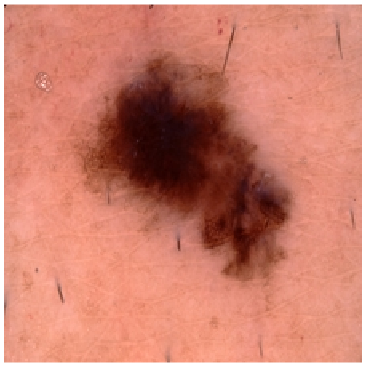
\includegraphics[width=2cm]{images/F22-A.png}} & 
        \adjustbox{valign=c}{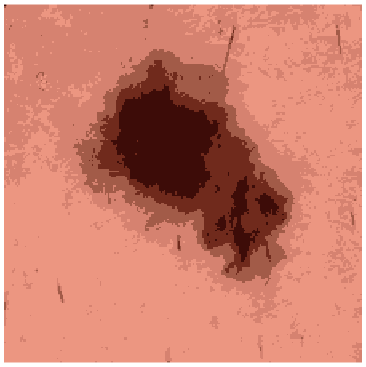
\includegraphics[width=2cm]{images/F22-B.png}} &
        \adjustbox{valign=c}{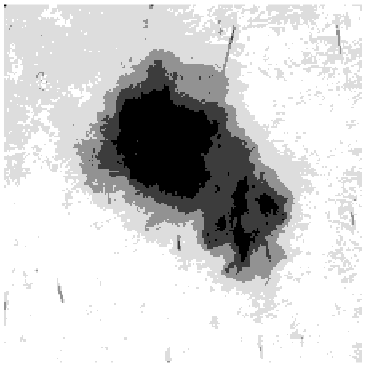
\includegraphics[width=2cm]{images/F22-C.png}} & 
        \adjustbox{valign=c}{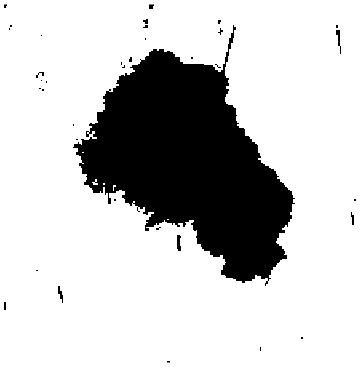
\includegraphics[width=1.5cm]{images/F22-D.png}} & 
		\adjustbox{valign=c}{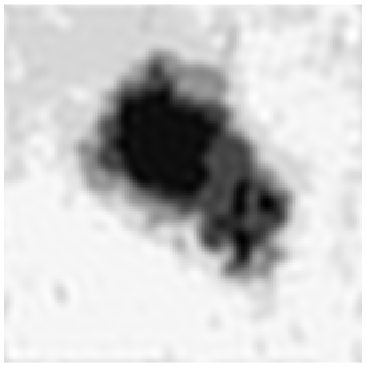
\includegraphics[width=2cm]{images/F22-E.png}} & 
        \adjustbox{valign=c}{
\includegraphics[width=1.2cm]{images/F22-F.png}} \\
        (a) & (b) & (c) & (d) & (e) & (f)\\
    \end{tabular}
    \caption{\footnotesize A: imagen en el modelo HSI, B: segmentación de color con K Menas, C: imagen B en blanco y negro, D: imagen C con valores ecualizados, E: imagen binaria de D, E: imagen paso bajas de C, F: imagen binaria de E}
    \label{fig22} 
\end{figure*}

% FIGURA 23
\begin{figure*}
    \centering
    \begin{tabular}{cccccc}
        \adjustbox{valign=c}{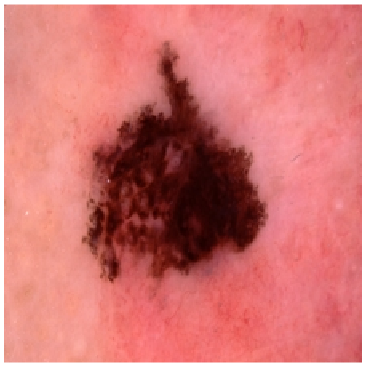
\includegraphics[width=2cm]{images/F23-A.png}} & 
        \adjustbox{valign=c}{\includegraphics[width=2cm]{images/F23-B.png}} &
        \adjustbox{valign=c}{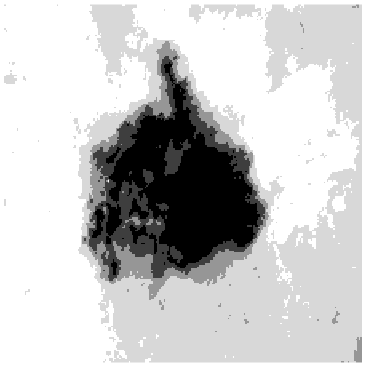
\includegraphics[width=2cm]{images/F23-C.png}} & 
        \adjustbox{valign=c}{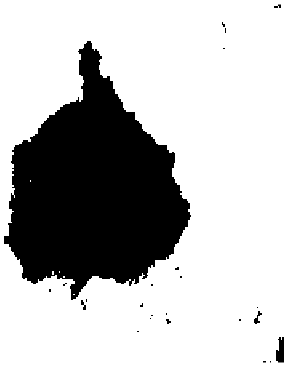
\includegraphics[width=1.5cm]{images/F23-D.png}} & 
		\adjustbox{valign=c}{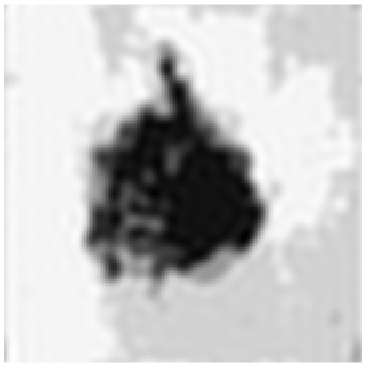
\includegraphics[width=2cm]{images/F23-E.png}} & 
        \adjustbox{valign=c}{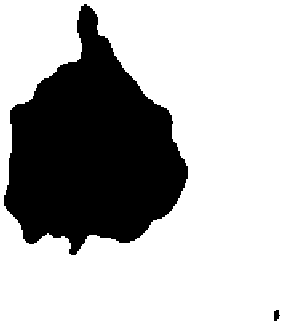
\includegraphics[width=1.5cm]{images/F23-F.png}} \\
        (a) & (b) & (c) & (d) & (e) & (f)\\
    \end{tabular}
    \caption{\footnotesize A: imagen en el modelo HSI, B: segmentación de color con K Menas, C: imagen B en blanco y negro, D: imagen C con valores ecualizados, E: imagen binaria de D, E: imagen paso bajas de C, F: imagen binaria de E}
    \label{fig23} 
\end{figure*}

% FIGURA 24
\begin{figure*}
    \centering
    \begin{tabular}{cccccc}
        \adjustbox{valign=c}{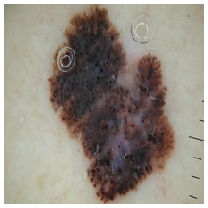
\includegraphics[width=2cm]{images/F24-A.png}} & 
        \adjustbox{valign=c}{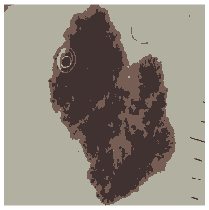
\includegraphics[width=2cm]{images/F24-B.png}} &
        \adjustbox{valign=c}{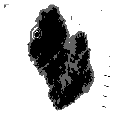
\includegraphics[width=2cm]{images/F24-C.png}} & 
        \adjustbox{valign=c}{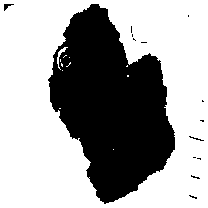
\includegraphics[width=1.5cm]{images/F24-D.png}} & 
		\adjustbox{valign=c}{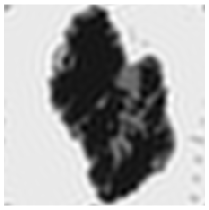
\includegraphics[width=2cm]{images/F24-E.png}} & 
        \adjustbox{valign=c}{
\includegraphics[width=1cm]{images/F24-F.png}} \\
        (a) & (b) & (c) & (d) & (e) & (f)\\
    \end{tabular}
    \caption{\footnotesize A: imagen en el modelo HSI, B: segmentación de color con K Menas, C: imagen B en blanco y negro, D: imagen C con valores ecualizados, E: imagen binaria de D, E: imagen paso bajas de C, F: imagen binaria de E}
    \label{fig24} 
\end{figure*}

% FIGURA 25
\begin{figure*}
    \centering
    \begin{tabular}{cccccc}
        \adjustbox{valign=c}{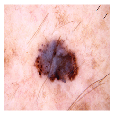
\includegraphics[width=2cm]{images/F25-A.png}} & 
        \adjustbox{valign=c}{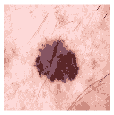
\includegraphics[width=2cm]{images/F25-B.png}} &
        \adjustbox{valign=c}{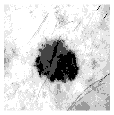
\includegraphics[width=2cm]{images/F25-C.png}} & 
        \adjustbox{valign=c}{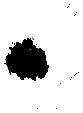
\includegraphics[width=1.5cm]{images/F25-D.png}} & 
		\adjustbox{valign=c}{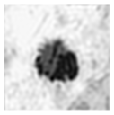
\includegraphics[width=2cm]{images/F25-E.png}} & 
        \adjustbox{valign=c}{
\includegraphics[width=1cm]{images/F25-F.png}} \\
        (a) & (b) & (c) & (d) & (e) & (f)\\
    \end{tabular}
    \caption{\footnotesize A: imagen en el modelo HSI, B: segmentación de color con K Menas, C: imagen B en blanco y negro, D: imagen C con valores ecualizados, E: imagen binaria de D, E: imagen paso bajas de C, F: imagen binaria de E}
    \label{fig25} 
\end{figure*}

% FIGURA 26
\begin{figure*}
    \centering
    \begin{tabular}{cccccc}
        \adjustbox{valign=c}{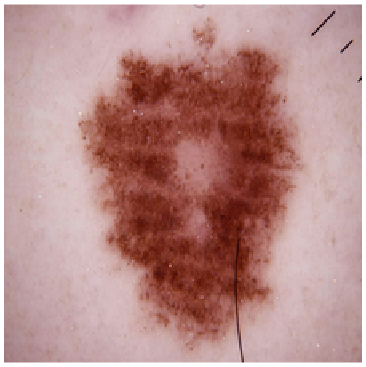
\includegraphics[width=2cm]{images/F26-A.png}} & 
        \adjustbox{valign=c}{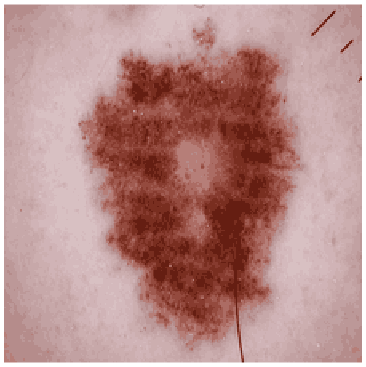
\includegraphics[width=2cm]{images/F26-B.png}} &
        \adjustbox{valign=c}{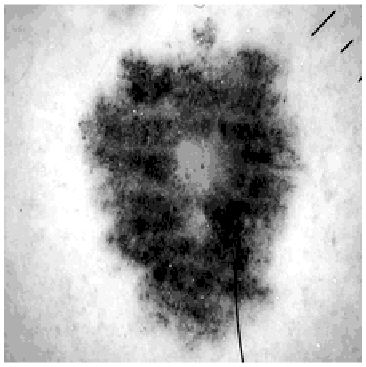
\includegraphics[width=2cm]{images/F26-C.png}} & 
        \adjustbox{valign=c}{
\includegraphics[width=1.5cm]{images/F26-D.png}} & 
		\adjustbox{valign=c}{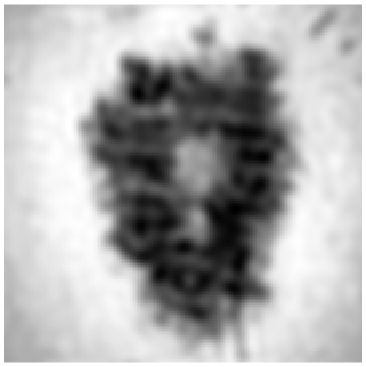
\includegraphics[width=2cm]{images/F26-E.png}} & 
        \adjustbox{valign=c}{\includegraphics[width=1cm]{images/F26-F.png}} \\
        (a) & (b) & (c) & (d) & (e) & (f)\\
    \end{tabular}
    \caption{\footnotesize A: imagen en el modelo HSI, B: segmentación de color con K Menas, C: imagen B en blanco y negro, D: imagen C con valores ecualizados, E: imagen binaria de D, E: imagen paso bajas de C, F: imagen binaria de E}
    \label{fig26} 
\end{figure*}




\clearpage

